\subsection{Reference resolution}
\subsubsection*{Setup}
In the final experiments, the agents are tasked to produced and understand referring expressions only based on the implicit human knowledge present in the scenes, as for example the attributes of the objects.
Opposed to the previous experiments, explicit human language information as human referring expressions or one-hot encoded attributes are avoided.
By this, the agents can't just reuse these human referring expressions, but need to learn to generate them themselves during the language games just based on the visual input.
This is done similarly to the single model reference resolution task, described in section \ref{sec:reference_resolution}.
As before, the sender has the same architecture as in the previous language games, encoding the bounding boxes of all objects.

The receiver is tasked to solve two tasks.
First, in the \textbf{coordinate reference resolver}, the agents are tasked to predict the center coordinates of the target object (see Figure \ref{fig:coordinate_predictor_game_architecture}).
The receiver is the same in both setups and is based on the \emph{reference resolver} + referring expressions, described in section \ref{sec:reference_resolution}.
Again, instead of the included LSTM, the receiver uses the \emph{EGG} LSTM with the hidden size $h_r=500$ and $e_r=100$ to encode the message.
The dimensions of the coordinate predictor are fixed to $c=2048$, based on the previous results.
% SD: Just thinking: would there be a more systematic way to compare all the models? Perhaps if you write the parameters in a table or a text that is parallel. Then you could simply say, modal A + these changes. It would be much clearer to the reader how all models are rerlated and it would be easier for the reader to follow.
% DK: TODO
The euclidean distance between the resulting prediction of the center point and the true center of the target object is calculated and the weights of both agents are adapted accordingly.

\begin{figure}[ht]
    \centering
    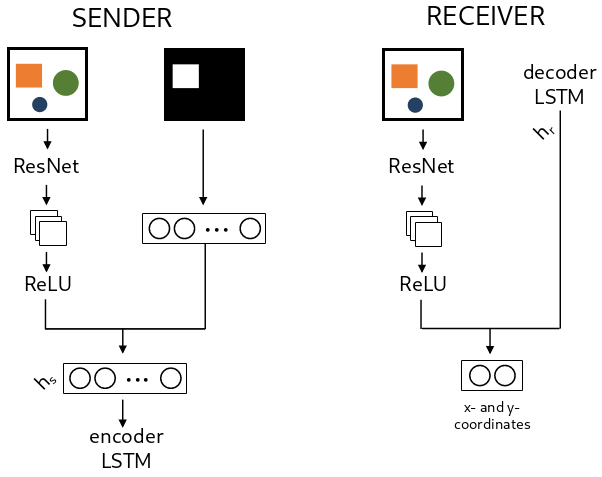
\includegraphics[width=.7\linewidth]{figures/arch_coordinate_predictor_game.png}
    \caption{Simplified architecture of the masked coordinate predictor game}
    \label{fig:coordinate_predictor_game_architecture}
    % SD: Again, why LSTM, are we inceremtally identifying the image while we are processing each input word?
    % DK: because it's a message sequence of discrete symbols (done)
\end{figure}

Secondly, in the \textbf{attention reference resolver}, the agents learn to point towards regions in the image, which is based on the \emph{attention reference resolver} described in section \ref{sec:reference_resolution}.
As before, the LSTM is replaced with the \emph{EGG} LSTM to parse the sender's message with the hidden size $h_r=500$ and $e_r=100$.
The dot product is calculated between each encoded region of the image and the encoded message, and the $softmax$ function is applied subsequently.
The loss is calculated using \emph{binary cross entropy} between the predictions and ground truth regions.

\cmtDK[inline]{figure}

The experiments are conducted with the following hyperparameters: a learning rate of $2\times10^{-4}$, a temperature for the Gumbel-Softmax relaxation of 1 and \emph{Adam} \citep{Kingma2015} as optimizer.
The following values for the variables are compared:
\begin{itemize}
    \item $|V|$: 2, 10, 16, 50, 100
    \item $n$: 1, 2, 3, 4,  6
\end{itemize}

As in section \ref{sec:reference_resolution}, the agents are trained first on the \emph{CLEVR single} dataset to understand if they are capable of predicting locations in an image together.
In a next step, the \emph{Dale-2}, \emph{Dale-5} and \emph{CLEVR color} datasets are used to test if the agents are able to first communicate a target object and second describe the target object discriminatively with a small vocabulary.
The same metrics are used to evaluate the results as described in \ref{sec:reference_resolution}.

\subsection*{Results}
In the final setup, the agents are tasked with communicating objects with fewer infused human knowledge.
Table \ref{tab:results_dale_predictor_game} shows the results for the setup, in which the sender is pointed towards the target object with a human description based on the GRE algorithm.
Hereby, the 'CLEVR single' dataset acts as a baseline, to test if the agents are able to predict coordinates of objects at all.
In every configuration of the variables, the agents achieve a very high performance.
The worst average distance across the test dataset is 10 pixels, which still points onto an object.
Also the accuracy, which evaluates how many guesses of the receiver were pointing onto an object reflects this fact.
All configuration achieve an accuracy higher than 96,7\%.
% SD: Just occured to me: how do we measure accuracy if we are predicting numbers (numeric prediction)?
% DK: same as in the experiments with one model (done)
This aligns also with the results from the single neural models, where the average distance was similarly low.
In general, this shows that the agents are able to predict coordinates together.
However, the question arises if the message by the sender has actually an effect on the receivers' decision, or if the receiver learns to point towards the target coordinates on his own and the message is ignored.
Having a look at the transferred messages, it in fact shows that the receiver learns to point towards the target object on its own.
% SD: But how could it do so if the visual data is randomly distribution. It must rely on the message as that is the only source of information.
% DK: it does it in the same way as the single model above (TODO)
As in the experiment before, all communicated messages contain the same symbol independent of the input image.

\begin{table}[ht]
    \centering
    \begin{tabular}{ccc|ccc|ccc|ccc}
        \toprule
              &         &         & \multicolumn{3}{c}{\textbf{CLEVR single}} & \multicolumn{3}{c}{\textbf{Dale-2}} & \multicolumn{3}{c}{\textbf{Dale-5}}                                                                                                       \\\cmidrule(lr){4-6}\cmidrule(lr){7-9}\cmidrule(lr){10-12}
        $|V|$ & $h_{s}$ & $h_{r}$ & \textbf{Dist.}                            & \textbf{Acc.}                       & \textbf{length}                     & \textbf{Dist.} & \textbf{Acc.} & \textbf{length} & \textbf{Dist.} & \textbf{Acc.} & \textbf{length} \\\midrule
        {10}  & {10}    & {10}    & {10,1}                                    & {98,5\%}                            & {1}                                 & {36,5}         & {19,9\%}      & {1}             & {45,7}         & {14,4\%}      & {1}             \\
        {13}  & {10}    & {10}    & {6}                                       & {99\%}                              & {0}                                 & {38}           & {20,4\%}      & {1}             & {47,3}         & {10,8\%}      & {1}             \\
        {20}  & {10}    & {10}    & {9,7}                                     & {96,7\%}                            & {1}                                 & {37,3}         & {21,2\%}      & {1}             & {47,3}         & {11,3\%}      & {0}             \\
        {100} & {10}    & {10}    & {7,7}                                     & {98,4\%}                            & {1}                                 & {40,4}         & {21,7\%}      & {1}             & {45,4}         & {10,8\%}      & {1}             \\
        {100} & {100}   & {100}   & {7,5}                                     & {96,9\%}                            & {1}                                 & {40,1}         & {17,8\%}      & {1}             & {44,3}         & {11,8\%}      & {0}             \\
        \bottomrule
    \end{tabular}
    \caption{Results of the description coordinate predictor: $|V|$ are different vocabulary sizes and $h$ hidden sizes.}
    \label{tab:results_dale_predictor_game}
\end{table}

When the experiments are run on the 'Dale-2' dataset, the results are much worse.
For the \emph{description coordinate predictor}, the average distance ranges from 36,5 pixels to 40,4 pixels.
The configuration with a vocabulary size of only 10 symbols fares the best, while a vocabulary of 100 symbols produces the worst results.
% SD: Remind the reader what is the size of the image so that they can interprert the distance relatively to that.
% DK: TODO
Still, the accuracy shows that around 19,9\% to 21,7\% of the guesses are on the target object.
Here, the configurations with higher vocabulary sizes fare slightly better, but the differences are very small and likely due to other factors.

The results for 'Dale-5' dataset are even worse, but are comparable with the results with a single neural model.
Apparently, the agents are not able to communicate the target object, and the predictions by the receiver are general in the middle of the image, which results in an average distance of around 45 to 50 pixels.
The differences of the mean distances are not very significant in this range, to allow an analysis of the different configurations.
% SD: I don't understand this
% DK: TODO

\begin{table}[ht]
    \centering
    \begin{tabular}{cccc|ccc|ccc|ccc}
        \toprule
              &         &         &         & \multicolumn{3}{c}{\textbf{CLEVR single}} & \multicolumn{3}{c}{\textbf{Dale-2}} & \multicolumn{3}{c}{\textbf{Dale-5}}                                                                                                       \\\cmidrule(lr){5-7}\cmidrule(lr){8-10}\cmidrule(lr){11-13}
        $|V|$ & $h_{s}$ & $h_{r}$ & $e_{s}$ & \textbf{Dist.}                            & \textbf{Acc.}                       & \textbf{length}                     & \textbf{Dist.} & \textbf{Acc.} & \textbf{length} & \textbf{Dist.} & \textbf{Acc.} & \textbf{length} \\\midrule
        {10}  & {10}    & {10}    & {1024}  & {10,8}                                    & {93,1\%}                            & {1}                                 & {34,8}         & {24,3\%}      & {0}             & {44,3}         & {11,8\%}      & {1}             \\
        {10}  & {10}    & {10}    & {512}   & {9,3}                                     & {92\%}                              & {1}                                 & {36,3}         & {19,9\%}      & {0,7}           & {45,9}         & {12,7\%}      & {1}             \\
        {13}  & {10}    & {10}    & {1024}  & {7,8}                                     & {96,8\%}                            & {1}                                 & {36,3}         & {20,2\%}      & {0}             & {45,4}         & {11,4\%}      & {1}             \\
        {20}  & {10}    & {10}    & {1024}  & {6,6}                                     & {98,3\%}                            & {1}                                 & {37,8}         & {16,1\%}      & {1}             & {45,2}         & {11\%}        & {1}             \\
        {100} & {10}    & {10}    & {1024}  & {5,2}                                     & {98,5\%}                            & {1}                                 & {37,4}         & {20,1\%}      & {1}             & {43,6}         & {16,7\%}      & {1}             \\
        {100} & {100}   & {100}   & {1024}  & {12,5}                                    & {92,1\%}                            & {1}                                 & {36,5}         & {20,7\%}      & {1}             & {44,6}         & {12,7\%}      & {1}             \\
        \bottomrule
    \end{tabular}
    \caption{Results of the masked coordinate predictor: $|V|$ are different vocabulary sizes, $h$ hidden sizes and $e$ embedding sizes.}
    \label{tab:results_masked_predictor_game}
\end{table}

Finally looking at the setup, when using the masked image as an input shows that the results are similarly bad as when using the encoded captions.
This is easily explainable with the emerged language.
For both the experiments using the encoded captions and the experiments using masked images as input, no meaningful symbols are transferred.
% SD: A bit gloomy result. Negative result is okay but then we need an explanation why this is so and have some ideas what to change. What we can learn from these results?
% DK: TODO
Following, the receiver needs to solve the task alone and the different setups of the sender don't play any role in the overall success.
% SD: This identifies that the problem lies in how the sender encodes the messages; what is its policy to generate longer strings or reuse the word. Without a policy the sender will never be motivated to encode longer messages and therefore rely on single-word expressions.
% SD: The second problem is the size of these networks. We should also test smaller embedding sizes than 10. Practice shows that the embedding sizes can be even several magnitues smaller than the vocabulary sizes, cf. the Bengio paper and word2vec.
% SD: The reason why the system is not performing well on the pointing task is that it does not have the right features to learn from. It ahs visual information WHAT these objects are (what do they look like) but they do not have information WHERE these objects are,. John Kelleher and I wrote an opiiuon piece about the lack of spatial knowledge required to model spatial descriptions in CNNs. The same problem is probably occuring here. Replacing the features or adding geometric features that would communicate geometric relations that allow pointing would improve the task and also we would expect that a vocabulary would emerge such that some words are more biased towards visual features (to identify objects) and some more to geometric features (to locate them), hence WHAT and WHERE.
% SD: J. D. Kelleher and S. Dobnik. What is not where: the challenge of integrating spatial representations into deep learning architectures. In S. Dobnik and S. Lappin, editors, Proceedings of the Conference on Logic and Machine Learning in Natural Language (LaML 2017), Gothenburg, 12 –13 June, volume 1 of CLASP Papers in Computational Linguistics, pages 41–52, Gothenburg, Sweden, November 2017. Department of Philosophy, Linguistics and Theory of Science (FLOV), University of Gothenburg, CLASP, Centre for Language and Studies in Probability.https://gup.ub.gu.se/publication/262970?lang=en
% SD: Overall, the thesis has a lot of potential if we could implement all this
% DK: TODO

When comparing these results to the neural models in Section \ref{sec:reference_resolution} that are not part of a language game, it can be seen that the metrics are very similar for all datasets.
The model was already not able to solve the task without the increased complexity of a language game.
This therefore indicates that the challenge for the agents doesn't lie in grounding the extracted features in new symbols, but already in extracting the features in the first place.